\documentclass[math,code]{amznotes}
%\usepackage[scheme=plain]{ctex}

\usepackage{lipsum}     % filler text

\begin{document}
    \tableofcontents

    \chapter{C\#.Net COM Addin}
	一直以来总是在使用VB6写comaddin,虽然用起来很顺手,但是VB6毕竟老了。于是乎有了向.net靠拢的思维。说实话,.net我也不是很喜欢,不过开
	发节省时间对我这种懒人还是可以的。C\#、VB.NET除了语法差异,对平常用来说基本一样。
	
	来吧,跟我一起造轮子吧(虽然很多高手很鄙视造轮子,我觉得造一遍轮子对新手练练手还是很有用的。)\cite{VBnet_ComAddin}
    \section{创建项目}
    
    VB6写comaddin是引用EXCEL、OFFICE,然后添加对 IRibbonExtensibility 、IDTExtensibility2 \cite{IDTExtensibility2}接口的引用,然后实现接口。C\#和VB.NET也一样。
    打开VST2022,新建项目,选择C\# ,类库(.net framework),为了兼容XP,框架选择 .net framework 4。
    
    % TODO: \usepackage{graphicx} required
%    \begin{figure}
%    	\centering
    	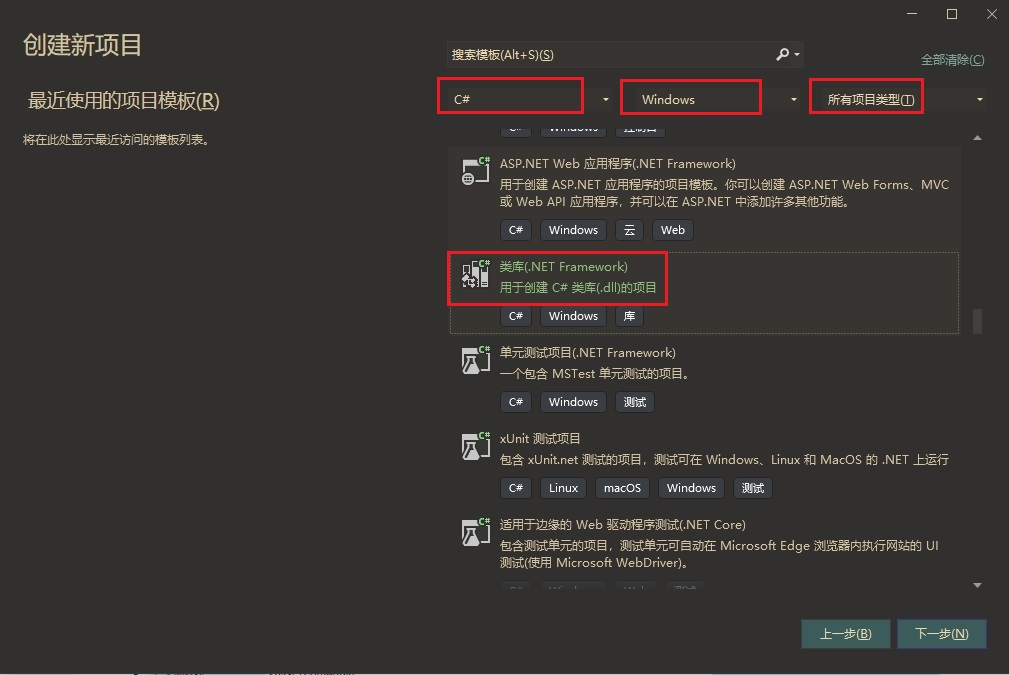
\includegraphics[width=0.5\linewidth]{pic/createProject}
%    	\caption{}
%    	\label{fig:createproject}
%    \end{figure}
    % TODO: \usepackage{graphicx} required
%    \begin{figure}
%    	\centering
    	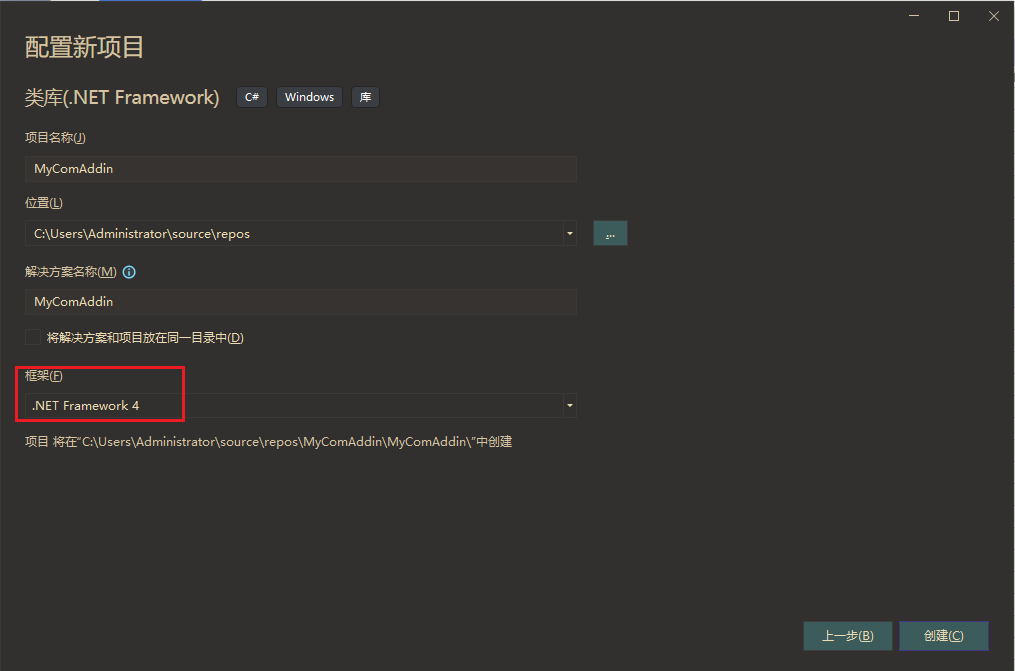
\includegraphics[width=0.5\linewidth]{pic/myComAddin}
%    	\caption{}
%    	\label{fig:mycomaddin}
%    \end{figure}
    
    将建立项目的默认Class1类名改成 Connect ,当然也可以自己随便起名,习惯这样。
    
	% TODO: \usepackage{graphicx} required
	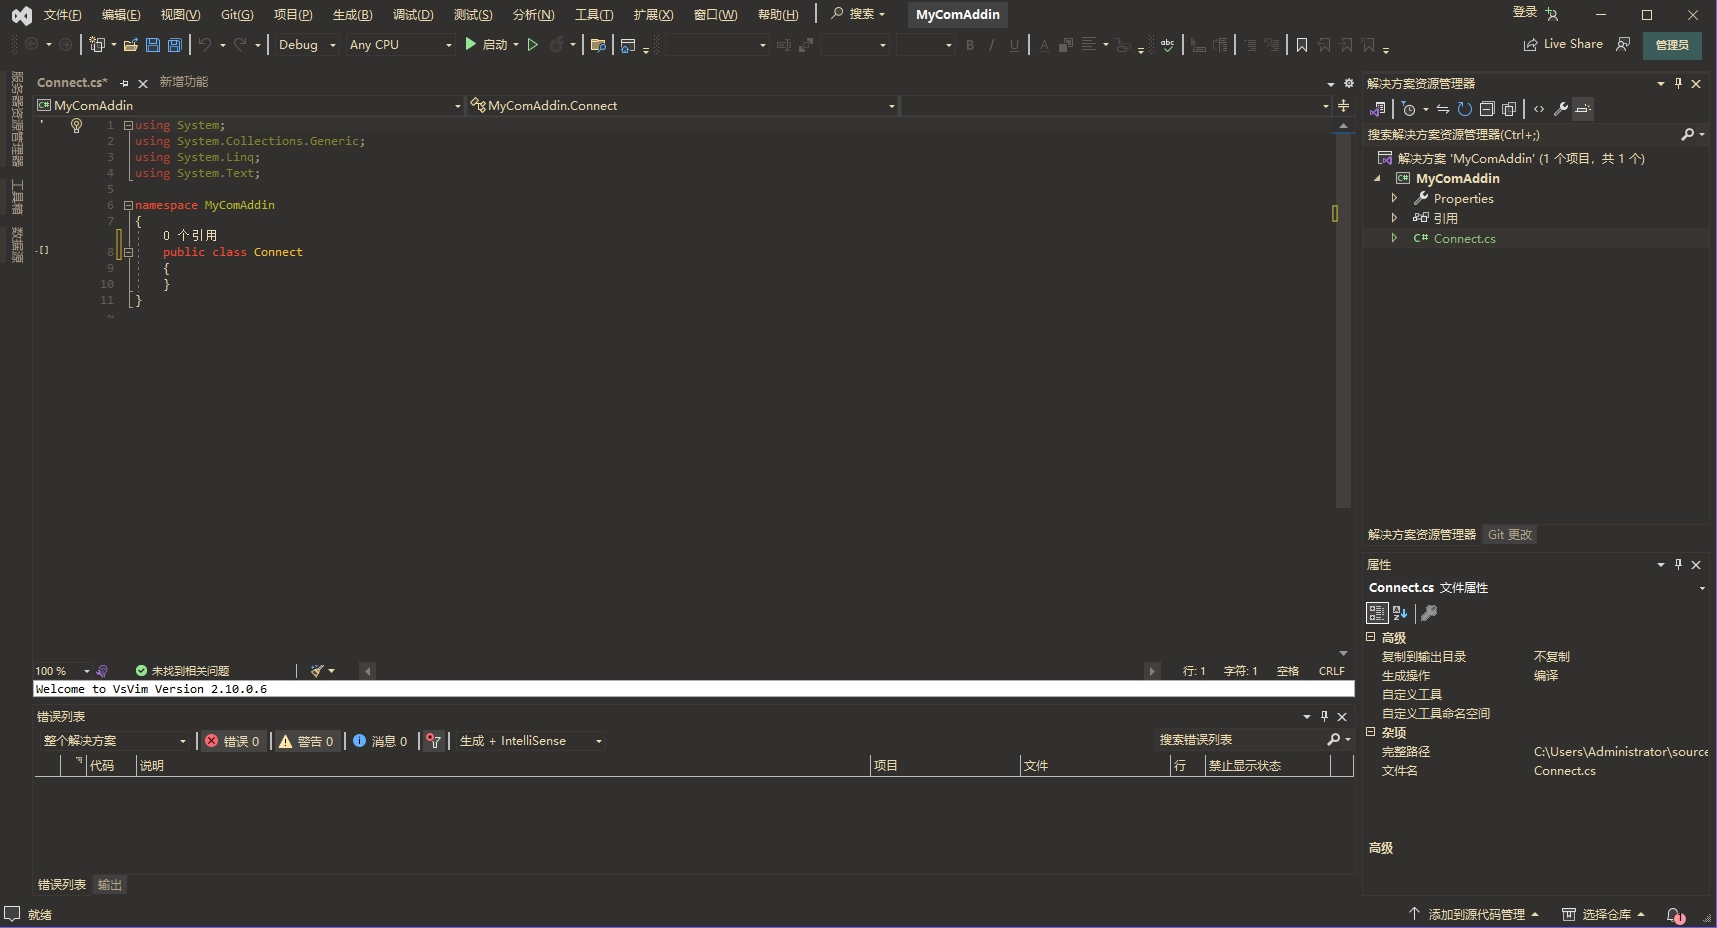
\includegraphics[width=1\linewidth]{pic/connect}
	\section{勾选COM可见、为COM互操作注册、签名、调试\cite{CS_OneNote}}
	\subsection{COM可见}
	在项目属性->“应用程序”页签中,选择程序集信息,勾选使程序集COM可见;
	
	% TODO: \usepackage{graphicx} required
	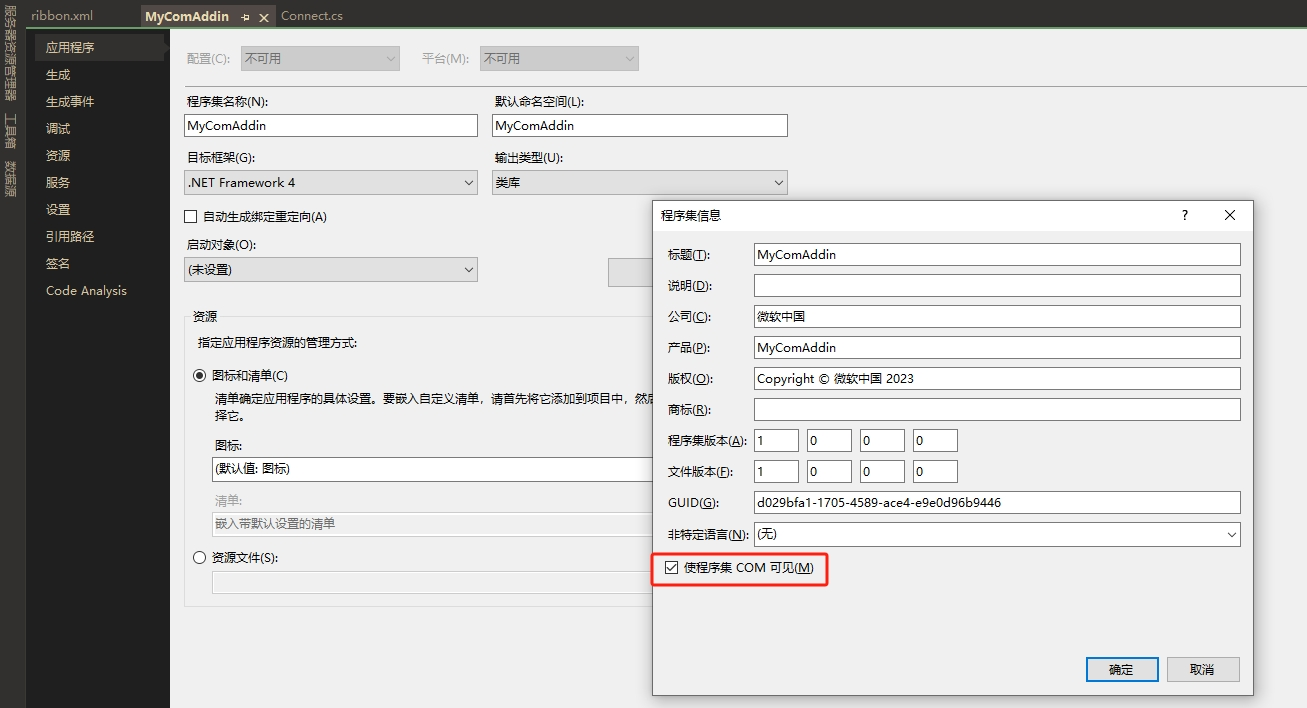
\includegraphics[width=0.9\linewidth]{pic/COM_visible}
	
	\subsection{为COM互操作注册}
	在项目属性->“生成”页签中,输出部分勾选“为COM互操作注册”;目标平台:“X64”;
	
	% TODO: \usepackage{graphicx} required
	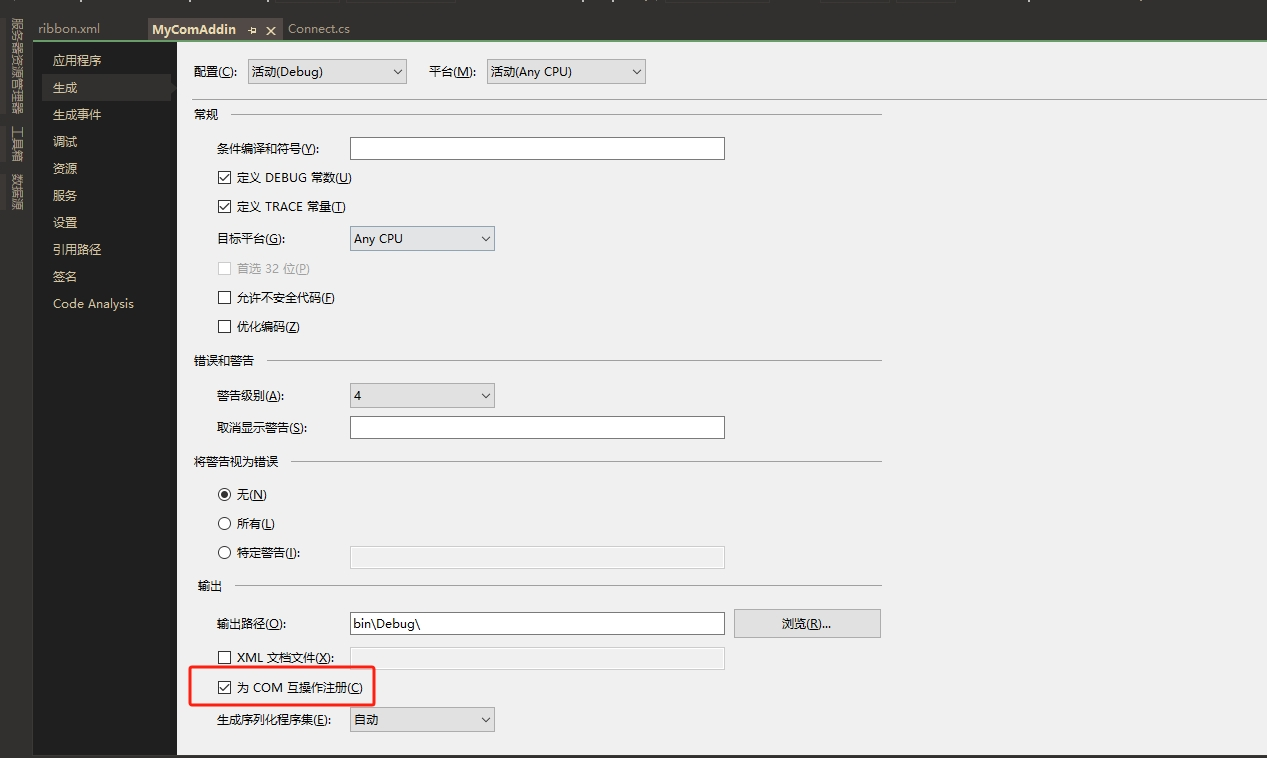
\includegraphics[width=0.9\linewidth]{pic/Com_interop}
		
	\subsection{调试} 选择项目属性,设置调试 ,启动外部程序,浏览到计算机里面安装的EXCEL.EXE 路径。
	
	% TODO: \usepackage{graphicx} required
	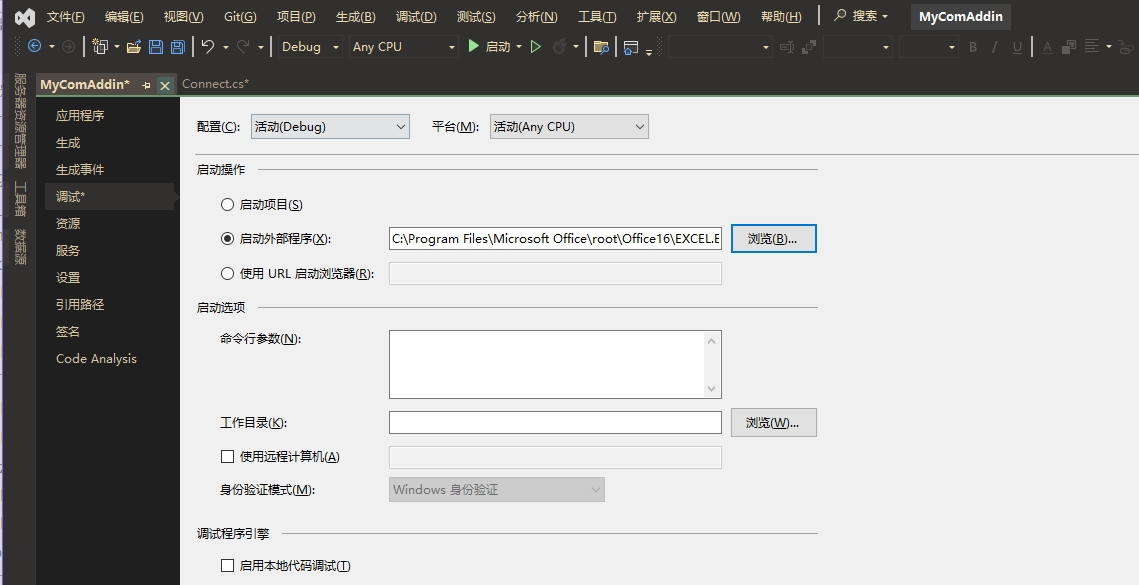
\includegraphics[width=0.9\linewidth]{pic/debug}
	
	\subsection{签名} 项目属性里面 签名,随便新增一个签名,使用密码保护密钥文件不用勾选;输入文件名称Conct后,会在右侧出现Cont.snk文件。
		
	% TODO: \usepackage{graphicx} required
	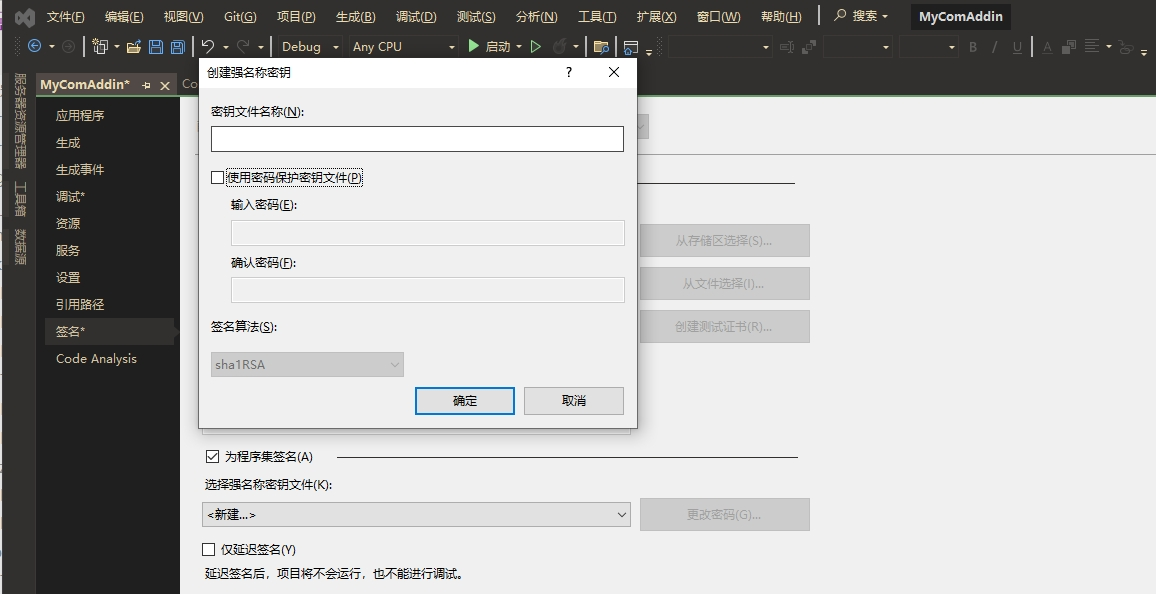
\includegraphics[width=0.9\linewidth]{pic/sign}
	
	\subsection{添加资源文件}
	
	右键新建项,数据,xml文件;xml内容如下:
	\begin{codebox}{XML示例}{xml}
	\begin{amzcode}{xml}
		<?xml version="1.0" encoding="utf-8" ?>
		<customUI xmlns="http://schemas.microsoft.com/office/2006/01/customui" loadImage="GetImage">
			<ribbon>
				<tabs>
					<tab id="tabCustom" label="Custom">
						<group id="groupHello" label="Hello">
							<button id="buttonHello" label="HelloExcel" size="large" screentip="Press this for a 'Hello World!' message" onAction="showHello" imageMso="HappyFace" />
						</group>
					</tab>
				</tabs>
			</ribbon>
		</customUI>		
	\end{amzcode}
	\end{codebox}
	相应xml标签的说明可以查看文档,重点说明下 \mintinline[]{xml}|onAction="showHello"| 和 \mintinline[]{xml}|imageMso="HappyFace"| 两个标记:
	\begin{itemize}[noitemsep]
		\item \mintinline[]{xml}|onAction="showHello"|,
		 Ribbon区域点击相应按钮或图片后执行的代码;具体实现由实际业务需求决定,测试例子见代码\ref{code:implementGetCustomUI};
		\item \mintinline[]{xml}|imageMso="HappyFace"| ,
		imageMso是系统内置图标,Value为图标的id;
	\end{itemize}
	
	% TODO: \usepackage{graphicx} required
	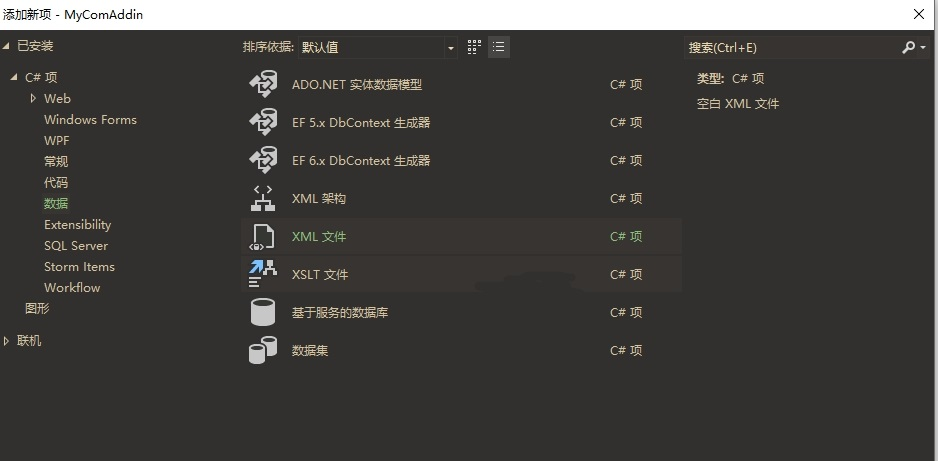
\includegraphics[width=0.9\linewidth]{pic/new_xml}	
	
	保存xml文件后,将xml文件拖入项目属性的资源页签,结果如下:
	
	% TODO: \usepackage{graphicx} required
	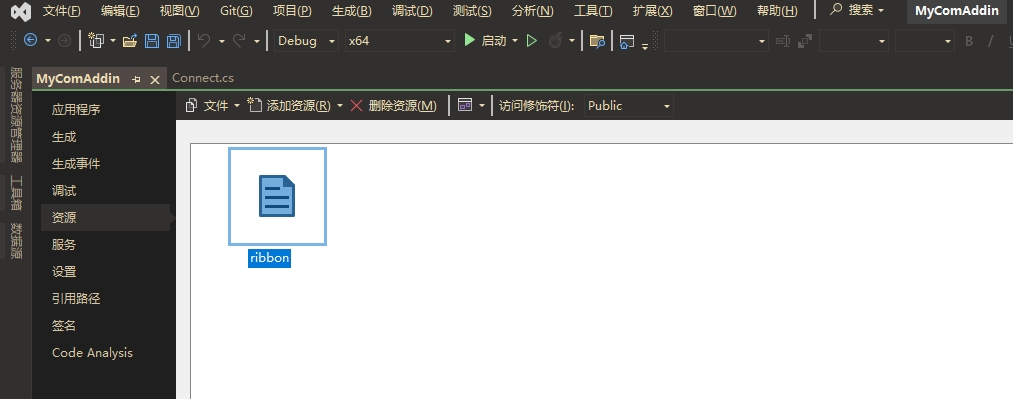
\includegraphics[width=0.9\linewidth]{pic/resource}
	
	重要一点,需要修改\mintinline{cs}{GetCustomUII(string RibbonID)}函数内容,具体参考\ref{code:implementGetCustomUI}%\ref{sec:implement_GetCustomUI}。
	
	\section{添加引用}
	接下来添加OFFICE和EXCEL引用,我一般习惯添加OFFICE14(EXCEL14 对应OFFICE2010、EXCEL15对应OFFICE2013、EXCEL16对应Office2016)。
	
	% TODO: \usepackage{graphicx} required
	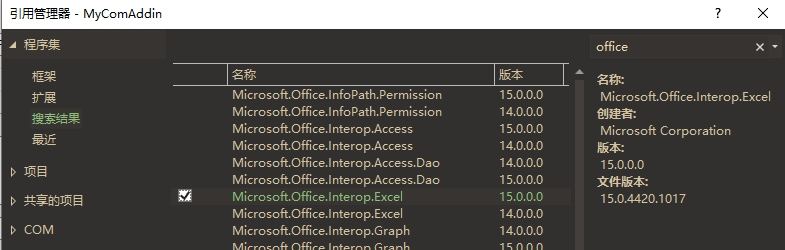
\includegraphics[width=0.9\linewidth]{pic/reference_excel}
	
	添加Microsoft.Office.Core、Microsoft.Office.Interop.Excel、Microsoft.Office.Tools、Office、Microsoft.Office.Tools.Common;System.Windows.Forms;	
	添加 Extensibility 引用(实现IDTExtensibility2 接口的),最结引用如下:
	
	% TODO: \usepackage{graphicx} required
	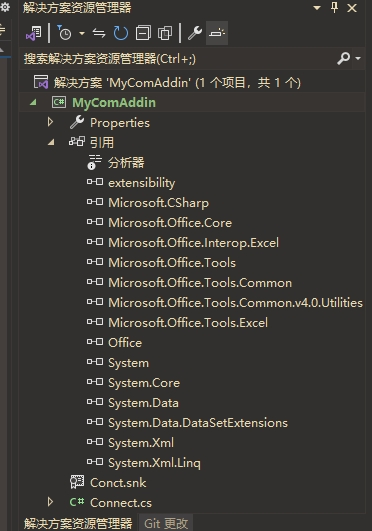
\includegraphics[]{pic/extensibility}
	
	在connect类顶部导入命名空间:
	\begin{codebox}{添加引用}{reference}
		\begin{amzcode}{cs}
			using System.Reflection;
			using System.Windows.Forms;
			using System.Runtime.InteropServices;
			using Excel = Microsoft.Office.Interop.Excel;
			using Extensibility;
			using System.Runtime.InteropServices; //为添加GUID和ProgID
			using Microsoft.Office.Core;
			using Microsoft.Office.Interop.Excel;
		\end{amzcode}
	\end{codebox}
	添加GUID和ProgID,可以使用菜单工具直接生成,复制过来;生成的GUID、ProgID是为后面系统注册表使用的;
	
	% TODO: \usepackage{graphicx} required
	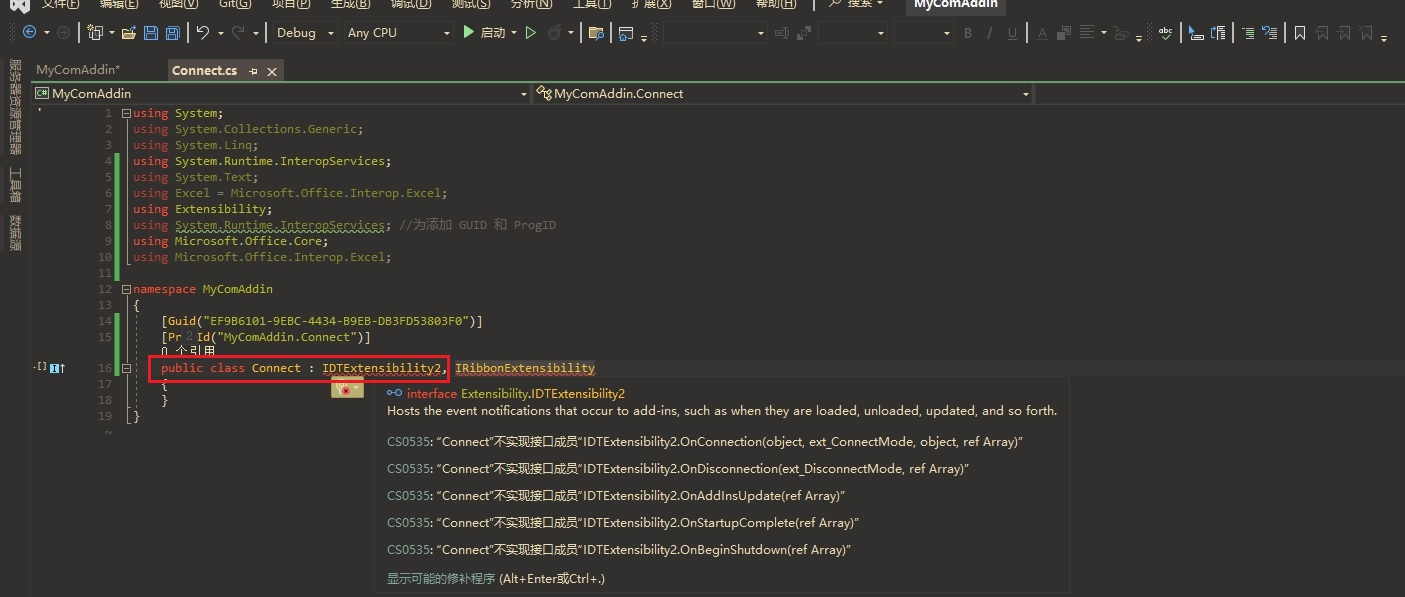
\includegraphics[width=0.9\linewidth]{pic/com_api}
	
	\section{实现接口}
	COM 外接程序是一个进程内 COM 服务器或 ActiveX 动态链接库 (DLL) ,可通过 IDTExensibility2 接口实现,如 Microsoft 外接程序设计器类型库 (Msaddndr.dll) 中所述。 所有 COM 加载项都继承自此接口,必须实现其五种方法中的每个方法。具体可参考微软官方API说明文档\cite{vst_comaddin}:
	\href{https://learn.microsoft.com/en-us/previous-versions/office/troubleshoot/office-developer/office-com-add-in-using-visual-c}{How to build an Office COM add-in by using Visual C\#.NET}
	
	看下红线报错,提示必须为接口实现。分别实现上述接口(下拉箭头,实现接口)。
	
	% TODO: \usepackage{graphicx} required
	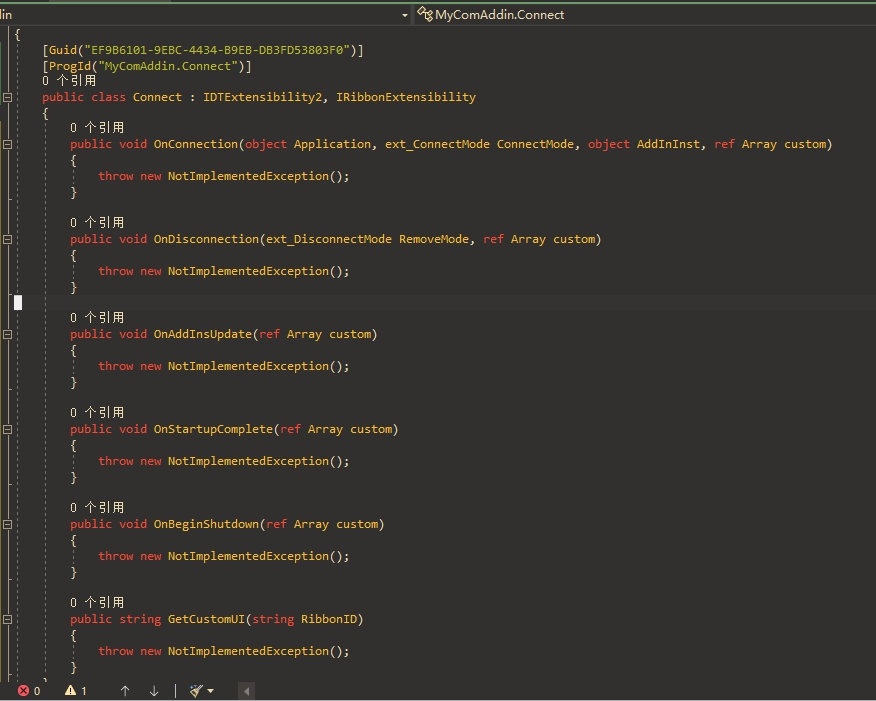
\includegraphics[width=0.9\linewidth]{pic/implement}
	
	删除所有的\mintinline[]{cs}|Throw New NotImplementedException()|;至此,一个空架子都搭起来了。
	\subsection{实现\mintinline[]{cs}|OnConnection|接口}
	程序入口就是\mintinline[]{cs}|OnConnection|,程序结束就是\mintinline{cs}{OnDisconnection}。
	在OnConnection 里面随便写一句\mintinline[]{cs}|MessageBox.Show("C#.NET ComAddin 你好 ");|;
	
	% TODO: \usepackage{graphicx} required
	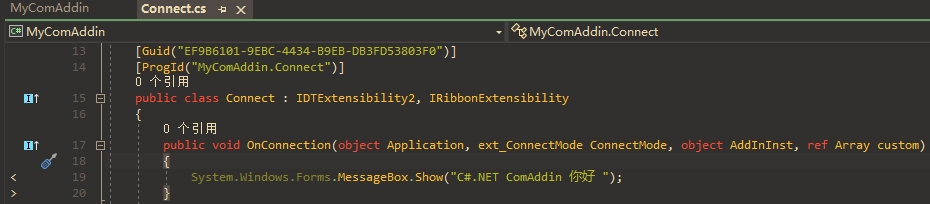
\includegraphics[width=0.9\linewidth]{pic/OnConnection}
	
	\subsection{实现\mintinline{cs}|GetCustomUI|接口}\label{sec:implement_GetCustomUI}
	GetCustomUI函数返回项目属性中资源文件;具体代码如下:
	\begin{codebox}{GetCustomUI}{implementGetCustomUI}
		\begin{amzcode}{cs}
			public void OnBeginShutdown(ref Array custom)
			{
			}
			
			public string GetCustomUI(string RibbonID)
			{
				return MyComAddin.Properties.Resources.ribbon;
			}
			public void showHello(IRibbonControl control)
			{
				
				MessageBox.Show("你点击了我哈哈!");
			}
		\end{amzcode}
	\end{codebox}
	
	\chapter{编译安装}
	
	\section{编译生成}
	在“生成”->“配置管理器”里面新建X64平台,然后点击生成,项目开始编译生成;成功后即可注册安装测试;
	
	% TODO: \usepackage{graphicx} required
	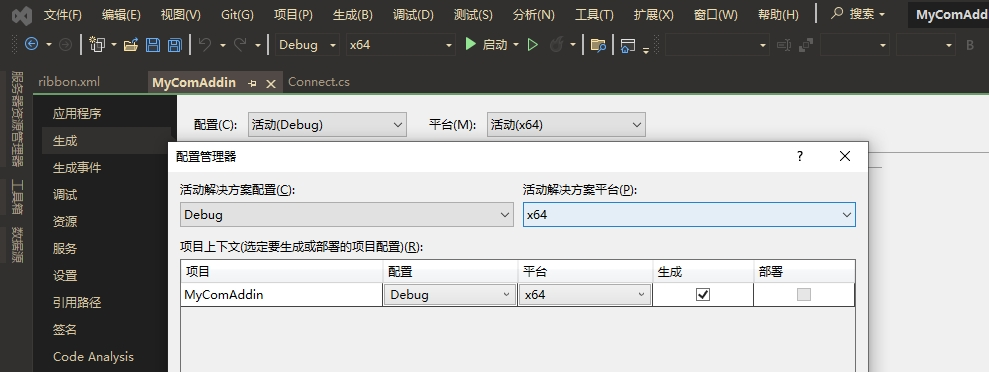
\includegraphics[width=0.9\linewidth]{pic/compileX64}
	
	\section{注册安装}
	项目右键,生成,然后在文件资源管理器中打开,找到\mintinline{bat}|bin\x64\Debug|文件夹 ,找到生成的MyComAddin文件,复制到\mintinline{bat}|windows\system32|(32位系
	统) 或者 \mintinline{bat}|windows\syswow64| (64位系统)文件夹里面,\\	
	然后开始菜单栏,附件里面 找到 CMD命令,右键以管理员身份打开,切换到\\ \mintinline[breaklines]{bat}|C:\Windows\Microsoft.NET\Framework\v4.0.30319| \\
	运行命令,
%	\begin{amzcode}{powershell}
	\begin{TermWin}[Width=13cm,Title={},Align=flush left]{}
regasm.exe /codebase c:\windows\syswow64\MyComAddin.dll /tlb c:\windows\syswow64\MyComAddin.tlb 
	\end{TermWin}
%	\end{amzcode}
	(具体路径自己写准确) ,注册32位OFFICE用。\\
	再次切换到 \mintinline[breaklines]{bat}|C:\Windows\Microsoft.NET\Framework64\v4.0.30319| 运行上述命令,注册64位OFFICE用。
	\begin{notebox}
		codebase 参数作用\cite{RegAsm_codebase}:
		/ codebase选项与您使用Regsvr32.exe注册COM服务器的方式完全等效.您必须选择DLL的特定位置,并将该位置的路径写入注册表.这是有风险的,COM服务器具有强大的DLL Hell问题,因为它们的注册是机器范围的.更新该DLL时,任何使用该服务器的应用程序都将受到影响.通常不会以一种好的方式,这经常会破坏未重新编译以使用更新的服务器的应用程序.
		
		.NET通过能够存储由[AssemblyVersion]选择的DLL的多个版本来改进.Windows并行缓存的完全等价物,即托管程序集的GAC.因此,未重建的旧应用程序将继续不受影响地运行,仍然可以使用旧的DLL.这是一个好方法.
		
		在忙于开发服务器时,建议使用/codebase.您可以跳过在GAC中注册DLL的额外必需步骤.忘记这样做很痛苦,你的更改似乎不起作用\cite{comAddin_LoadFailure,VSTO_comAddin_LoadFailure},因为测试应用程序将加载旧版本.当你使用/ codebase时,Regasm会显示一个警告,警告你关于DLL Hell的潜力,你可以忽略它.
		
		当您让Visual Studio通过"项目">"属性">"构建"选项卡"注册COM互操作"复选框进行注册时,您将获得Regasm/codebase/tlb的完全等效项.这样做更为可取,因为它还确保了旧版本的程序集未注册,从而避免了注册表污染.但VS必须运行升级才能写入注册表.
		
		使用隔离COM(又名"无注册表COM")是最好的方法.它允许您将COM服务器的副本存储在与客户端程序相同的目录中,而您根本不需要注册它.然而,这需要修改客户端程序,如果您对客户端应用程序没有任何控制权,或者如果它是其他人喜欢混淆的那种应用程序,则很难.例如,Microsoft Office应用程序.
	\end{notebox}
	当然这样还没完,显示注册成功了,你打开EXCEL却看不到,因为还有注册表要写入。新建一个\verb|install.reg|文件,写入如下注册表项目\cite{CS_WPS}:
	\begin{codebox}{注册dll}{registry}
		\begin{amzcode}{registry}
	Windows Registry Editor Version 5.00
	[HKEY_CURRENT_USER\SOFTWARE\Microsoft\Office\EXCEL\Addins\MyComAddin.Connect]
	"FriendlyName"="MyComAddin"
	"Description"="MyComAddin"
	"LoadBehavior"=dword:00000003
	"CommandLineSafe"=dword:00000001
	[HKEY_CURRENT_USER\Software\Kingsoft\Office\ET\AddinsWL]
	"MyComAddin.Connect"=""
		\end{amzcode}
	\end{codebox}
	卸载插件:
	\begin{codebox}{反注册dll}{unregistry}
		\begin{amzcode}{registry}
			Windows Registry Editor Version 5.00
			[-HKEY_CURRENT_USER\SOFTWARE\Microsoft\Office\EXCEL\Addins\MyComAddin.Connect]
			[HKEY_CURRENT_USER\Software\Kingsoft\Office\ET\AddinsWL]
			"MyComAddin.Connect"=-
		\end{amzcode}
	\end{codebox}
	再创建安装bat:
	\begin{codebox}{安装}{install}
		\begin{amzcode}{bat}
	@echo off
	
	@set baseDir="%cd%"
	Echo.
	Echo 【1】导入注册表
	regedit /s %baseDir%\install.reg
	Echo.
	Echo 【2】注册类型
	C:\Windows\Microsoft.NET\Framework64\v4.0.30319\RegAsm.exe /codebase %baseDir%\MyComAddin.dll /tlb:%baseDir%\MyComAddin.tlb
	Echo.
	Echo 【3】添加程序集到GAC
	@SETGACUTIL="%baseDir%\NETFX 4.0 Tools\gacutil.exe"
	%GACUTIL%-i %baseDir%\WPP_test.dll
	%GACUTIL%-i %baseDir%\PowerPoint.dll
	%GACUTIL%-i %baseDir%\Office.dll
	pause
		\end{amzcode}
	\end{codebox}
	创建卸载bat:
	\begin{codebox}{卸载}{uninstall}
		\begin{amzcode}{bat}
			@echo off 
			@set baseDir="%cd%" 
			Echo. 
			Echo 【1】从缓存中移除程序集 
			@SETGACUTIL="%baseDir%\NETFX 4.0 Tools\gacutil.exe" 
			rd /s /QC:\Windows\Microsoft.NET\assembly\GAC_MSIL\WPP_test 
			rd /s /QC:\Windows\Microsoft.NET\assembly\GAC_MSIL\PowerPoint 
			rd /s /QC:\Windows\Microsoft.NET\assembly\GAC_MSIL\Office 
			Echo.
			
			Echo 【2】注销类型 
			C:\Windows\Microsoft.NET\Framework64\v4.0.30319\RegAsm.exe /u %baseDir%\MyComAddin.dll /tlb:%baseDir%\MyComAddin.tlb 
			Echo.
			
			Echo 【3】清除注册表 
			regedit /s %baseDir%\uninstall.reg 
			pause
		\end{amzcode}
	\end{codebox}
	至此全部完成,打开EXCEL会看到如下效果。 
	\section{反注册\cite{COM_unregistry}}
	How to Unregister a DLL using RegAsm.exe?\cite{RegAsm_unregiste}
	
	To run the tool, use Visual Studio Developer Command Prompt or Visual Studio Developer PowerShell. Unregistering a DLL using RegAsm.exe is so easy as registering.
	
	Open Command Prompt and run the following command replacing the <dllfilename> name with the name you want to unregister.
	\begin{amzcode}{bat}
	regasm /u <dllfilename>.dll
	\end{amzcode}
	To unregister the DLL completely, you have to unregister the type library of the DLL too. To do so, run the following command.
	\begin{amzcode}{bat}
	regasm <dllfilename> /tlb /unregister
	\end{amzcode}
	
	\section{使用插件布署安装}
	
	
\chapter{VSTO开发}
	\section{Setup Project}
	\section{inno setup 打包vsto项目}
    \amzindex
	\bibliographystyle{unsrt}
	\bibliography{ref}
\end{document}
